%
% Dataontwerp
%

\chapter{Dataontwerp}

\begin{figure}[h!]
	\centering
		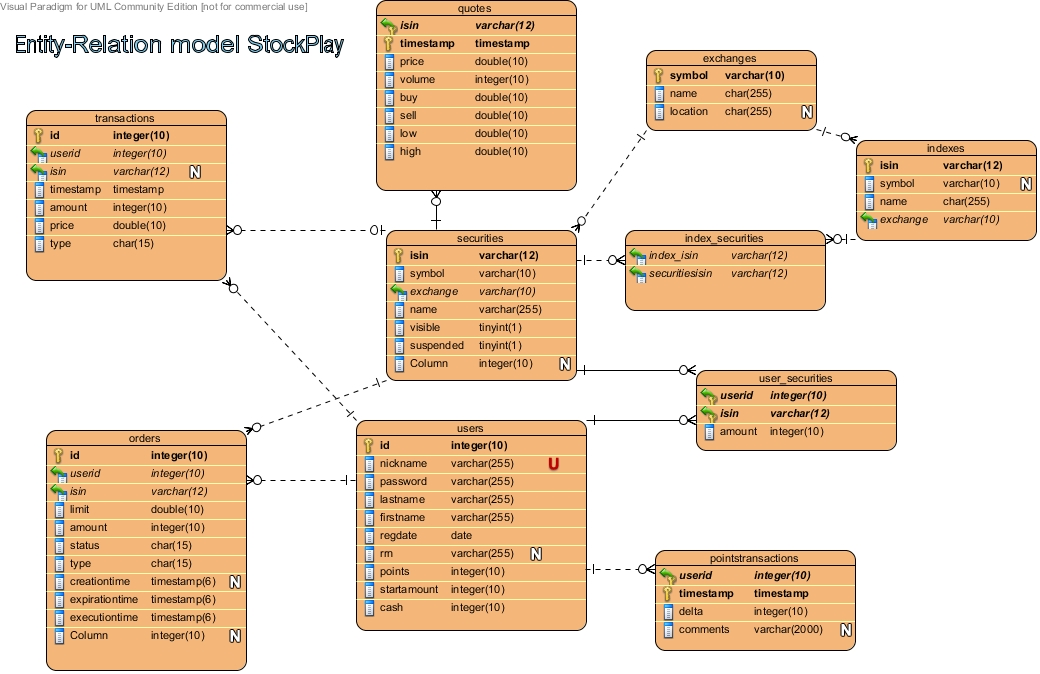
\includegraphics[width=0.5\textwidth]{images/realisatie/ER_Diagram}
	\caption{Entity-relationship model.}
\end{figure}

\section{Ontwerp backend}
\todo{dit hoort hier niet}
De klassen die de persistente data uit de database moeten weergeven staan opgesomd in onderstaand klassendiagram:

\begin{figure}[h!]
	\centering
		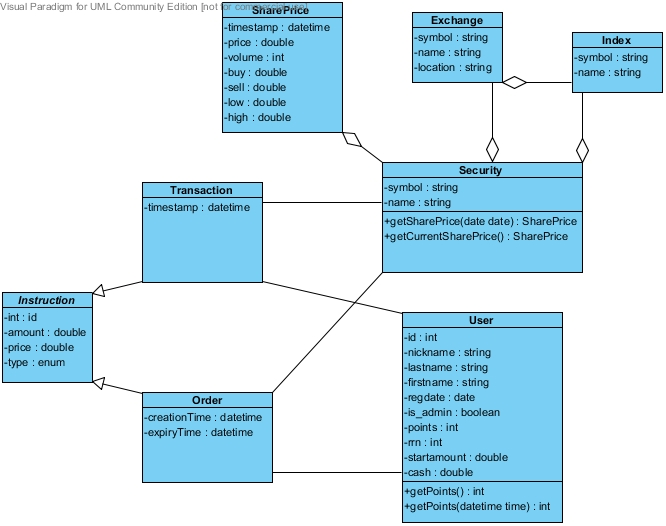
\includegraphics[width=0.5\textwidth]{images/realisatie/Class_Diagram}
	\caption{Klassendiagram persistente data in backend.}
\end{figure}

Op onze databank hebben we ook een aantal triggers. De punten mogen niet zomaar mogen aangepast in de gebruikerstabel. Elke wijziging gebeurt via de pointshistory tabel. Het toevoegen van een nieuw record daarin zorgt ervoor dat een trigger de delta waarde in de pointshistory optelt bij de punten in de userstabel. Zodoende hebben we een cache van het puntentotaal die we snel kunnen raadplegen.

Ook bij het omzetten van een order naar een transactie wordt een trigger geactiveerd die nakijkt of de gebruiker wel voldoende cash positie bezit.

De cash positie van een gebruiker kan niet zomaar aangepast worden, dit wordt ook beveiligd met een trigger.


%
% Procedureontwerp
%

\chapter{Procedureontwerp}

\section{XML-RPC interface}

Zoals vermeld bij het technisch ontwerp, gebruiken we het XML-RPC protocol als communicatiemiddel tussen de backend en zijn interfaces. Hiertoe moeten we de set aan functies vastleggen die een client kan uitvoeren, en de bijhorende signatuur documenteren.

Aangezien XML-RPC geen ondersteuning biedt voor namespaces of andere vormen van functieorganisatie, hanteren we zelf een mechanisme om dit te bekomen: een methode-naam bestaat altijd uit twee delen, gescheiden door een punt. Het deel voor het scheidingsteken duidt het pakket aan, het deel erna de methode die we willen oproepen.
Zo delen we de backend op in de volgende drie primaire klassen:
\begin{itemize}
\item{System: functionaliteit voor beheer en de statusinformatie van het systeem.}
\item{User: beheer van gebruikers en ophalen gebruikersinformatie.}
\item{Finance: functionaliteit gerelateerd aan het beurswezen.}
\end{itemize}
Hogere-orde klassen zijn eventueel ook mogelijk (zoals \emph{System.Database}), maar niet verplicht. De semantiek is daarbij identiek aan primaire klassen, met een punt als scheidingsteken.

\subsection{Algemene foutcodes}

De XML-RPC specificatie biedt ook ondersteuning voor foutberichten, in de form van een bericht met een $<$fault$>$ tag. Die tag moet steeds twee $<$member$>$ tags bevatten, namelijk een foutcode $<$faultCode$>$ van het integer type, en een foutbericht $<$faultString$>$ van het string type. Elk van de klassen kan zo specifieke foutmeldingen vastleggen.
Maar er zijn ook generieke foutmeldingen, die van toepassing zijn op alle klassen. Deze foutmeldingen, waarvan de foutcode in het bereik $[0, 100[$ valt, worden hieronder beschreven:

\begin{table}
\begin{tabular}{| c p{5cm} p{7cm} |}
	\hline
	Foutcode & Foutbericht & Controle \\
	\hline
	
	0 & Internal Failure & Verifieer de status van de backend, de log kan hierbij helpen. \\
	\hline
	
	$[1-10[$ & \emph{Subsystem failures.} & \\
	1 & Database Failure & Er is een probleem met de database (onbeschikbaar, corrupt, ...), zie de log voor meer details. \\
	2 & Scraper Failure & Er is een probleem met de scraper (onbeschikbaar, uitgevallen, ...), zie de log voor meer details. \\
	\hline
	
	$[10-20[$ & \emph{Service issues.} & \\
	10 & Service Unavailable & De backend kan tijdelijk niet gebruikt worden (werkzaamheden, overloaded, ...). \\
	11 & Unauthorized & Meld u aan vooraleer deze functie te gebruiken. \\
	\hline
	
	$[20-30[$ & \emph{Invocation issues.} & \\
	20 & Version Not Supported & De client gebruikt een verkeerd communicatieprotocol. \\
	21 & Not Found & Methode niet gevonden, verifieer de schrijfwijze en de klasse. \\
	21 & Bad Request & Probleem met de parameters, controleer het gebruik van de methode. \\
	\hline
\end{tabular}
\caption{Generieke foutcodes in het backend-protocol.}
\end{table}

\subsection{Authenticatie en autorisatie}

Aangezien het XML-RPC protocol gebruik maakt van het HTTP-protocol, kunnen we diens functionaliteit gebruiken om authenticatie te bekomen. Daartoe zullen we gebruik maken van \emph{basic authentication}, waarbij de client indien gevraagd een gebruikersnaam en wachtwoord naar de server doorstuurd.
\todo{Dit is tijdelijk - hoe bedoel je tijdelijk? Hier waren we toch al over eens denk ik? - Laur}

Afhankelijk van de mogelijkheden van het XML-RPC pakket dat we in de backend gebruiken (Apache XML-RPC), kan dit op twee manieren verlopen. Indien de bibliotheek ondersteuning biedt voor het on-demand inschakelen van authenticatie gebaseerd op de ontvangen request, kunnen we zo wanneer benodigd \emph{basic authentication} inschakelen en de webserver zelf een HTTP-401 laten terugsturen. Hiervoor is dan geen extra code in de backend benodigd.
Als deze optie niet dynamisch ingeschakeld kan worden, zullen we zelf een eigen foutmelding moeten terugsturen die aanduidt dat authorisatie benodigd is. Als de client zo een $<$fault$>$-bericht ontvangt, zal die een nieuwe XML-RPC socket openen op een alternatieve URL (bijvoorbeeld \texttt{http://server.hogent.be/authenticated}). Aangezien de URL nu verschillend is, kunnen we de webserver in de backend zodanig configureren dat authenticatie vereist is voor die zone. Zo bekomen we eveneens verplichte authenticatie voor bepaalde methodes, maar dit door ze enkel beschikbaar te stellen in een subset van het serverdomein. Dit vereist echter enige extra code in de backend.

Autorisatie wordt bepaald door een bitmap. Mogelijke rechten zijn:
\begin{itemize}
\item{1: securities bekijken}
\item{2: rankings bekijken}
\item{4: user-profielen bekijken}
\item{8: securities verhandelen}
\item{16: gebruikers wijzigen of verwijderen}
\item{32: securities wijzigen of verwijderen}
\item{64: quotes toevoegen of wijzigen}
\end{itemize}

Hoewel een administrator gebruikersprofielen (en bijhorende autorisatiebits) manueel kan aanpassen, kennen we de volgende categorieën gebruikers:
\begin{table}
\begin{center}
\begin{tabular}{| c | r |}
	\hline
	\textbf{Gebruiker} & \textbf{Rechten} \\
	\hline
	Gast & 1 \\
	Speler & 1+2+4+8 = 15 \\
	Administrator & 1+2+4+8+16+32 = 63 \\
	Scraper & 1+64 = 65 \\
	\hline
\end{tabular}
\caption{Standaard gebruikersklassen en bijhorende rechten.}
\end{center}
\end{table}

\subsection{System-klasse}

Deze klasse biedt de client mogelijkheden om het systeem te beheren. Zoals het ophalen van informatie, wijzigen van configuraties, en (her)starten of stoppen van bepaalde subsystemen.

\function{Backend.Status}
	{ status van de backend ophalen }
	{ geen }
	{ integer die de status beschrijft:
		\begin{itemize}
		\item{0: maintenance-mode}
		\item{1: geen problemen gemeld}
		\end{itemize} }
	{ administrator-rechten }

\function{Backend.Stats}
	{ backend-statistieken ophalen }
	{ geen }
	{ struct met statistieken:
		\begin{itemize}
		\item{users: aantal gebruikers online}
		\item{req: aantal verwerkte XML-RPC requests sinds de start}
		\item{uptime: hoe lang de backend al draait}
		\end{itemize} }
	{ administrator-rechten }

\function{Backend.Restart}
	{ de backend opnieuw opstarten }
	{ geen }
	{ bool die indiceert of de actie succesvol was }
	{ administrator-rechten }

\function{Backend.Stop}
	{ de backend stoppen }
	{ geen }
	{ bool die indiceert of de actie succesvol was }
	{ administrator-rechten }

\function{Database.Status}
	{ informatie van de database ophalen }
	{ geen }
	{ integer die status beschrijft:
		\begin{itemize}
		\item{0: er kon geen verbinding naar de databank gelegd worden}
		\item{1: succesvol verbonden met de database}
		\end{itemize} }
	{ administrator-rechten benodigd}

\function{Database.Stats}
	{ database-statistieken ophalen. Dit zijn de statistieken geleverd door de databank zelf, ze zijn dus niet beperkt tot acties ondernomen door de backend }
	{ geen }
	{ struct met statistieken:
		\begin{itemize}
		\item{queries: aantal uitgevoerde queries}
		\item{uptime: hoe lang de databank al draait}
		\item{traffic: hoeveelheid data verzonden en ontvangen}
		\item{slow\_queries: aantal queries die teveel uitvoeringstijd vergden}
		\end{itemize} }
	{ administrator-rechten }

\function{Scraper.Status}
	{ status van de scraper ophalen }
	{ geen }
	{ integer die status beschrijft:
		\begin{itemize}
		\item{0: niet geactiveerd}
		\item{1: inactief}
		\item{2: bezig met data-mining}
		\end{itemize} }
	{ administrator-rechten }

\function{Scraper.Stats}
	{ scraper-statistieken ophalen }
	{ geen }
	{ struct met statistieken:
		\begin{itemize}
		\item{executes: aantal voltooide plugin-uitvoeringen}
		\item{uptime: hoe lang de scraper al draait}
		\item{traffic: hoeveelheid data verzonden en ontvangen}
		\item{plugins: aantal geactiveerde plugins}
		\item{securities: aantal beschikbare effecten}
		\item{exchanges: aantal beschikbare beurzen}
		\item{indexes: aantal beschikbare indexen}
		\item{delay: tijd tot de volgende plugin-uitvoering}
		\item{memory: geheugengebruik}
		\end{itemize} }
	{ administrator-rechten }

\function{Scraper.Restart}
	{ de scraper herstarten }
	{ geen }
	{ bool die indiceert of de actie succesvol was }
	{ administrator-rechten }

\function{Scraper.Stop}
	{ de scraper permanent stilleggen }
	{ geen }
	{ bool die indiceert of de actie succesvol was }
	{ administrator-rechten }


\subsection{User-klasse}

Hier vindt men de nodige methodes terug om gebruikers te beheren. Dit is echter niet beperkt tot de administrator: ook gebruikers zelf kunnen hun eigen profiel (in beperktere mate) beheren.

\function{List}
	{ lijst met publieke informatie opvragen van de gebruikers }
	{ een filter, met de volgende mogelijke sleutels:
		\begin{itemize}
		\item{nickname: gebruikersnaam}
		\item{regdate: datum van registratie}
		\item{points: aantal behaalde punten}
		\end{itemize} }
	{ een lijst met structs:
		\begin{itemize}
		\item{id: gebruikers-id}
		\item{nickname: gebruikersnaam}
		\item{regdate: datum van registratie}
		\item{points: aantal behaalde punten}
		\end{itemize} }
	{ geen benodigd }

\function{Details}
	{ lijst met publieke informatie opvragen van een gebruiker }
	{ een filter, met de volgende mogelijke sleutels:
		\begin{itemize}
		\item{id: een gebruikers-id}
		\end{itemize} }
	{ een lijst met structs:
		\begin{itemize}
		\item{id: gebruikers-id}
		\item{firstName: voornaam}
		\item{lastName: achternaam}
		\item{rrn: rijksregisternummer (nodig voor de eid authenticatie)}
		\item{cash: huidige cashpositie}
		\item{startkapitaal: start kapitaal}
		\end{itemize} }
	{ administrator-rechten of identificatie als de gebruiker beschreven is in het 'id' veld van de filter }

\todo{specifieke foutcode genereren} 
\function{Create}
	{ aanmaken van een nieuwe gebruiker }
	{ struct met de gebruikersinformatie:
		\begin{itemize}
		\item{}
		\end{itemize} }
	{ id van de aangemaakte gebruiker }
	{ administrator-rechten }

\function{Modify}
	{ wijzigen van een bestaande gebruiker }
	{ een filter die gebruikers selecteert, en een struct met de te-wijzigen gebruikersinformatie:
		\begin{itemize}
		\item{}
		\end{itemize} }
	{ een boolean die aangeeft of de actie al dan niet gelukt is }
	{ administrator-rechten of identificatie als de gebruiker beschreven is in het 'id' veld van de filter }

\function{Remove}
	{ verwijderen van een bestaande gebruiker }
	{ een filter die gebruikers selecteert }
	{ een boolean die aangeeft of de actie al dan niet gelukt is }
	{ administrator-rechten }

\function{Portfolio.List}
	{ basisinformatie van effecten in bezit opsommen (gebruik de functie Finance.Security.Details voor meer informatie) }
	{ een filter, met de volgende mogelijke sleutels:
		\begin{itemize}
		\item{id: een gebruikers-id}
		\end{itemize} }
	{ array van structs met basisinformatie van de effecten:
		\begin{itemize}
		\item{symbool: identificatiecode van het aandeel}
		\end{itemize} }
	{ administrator-rechten of identificatie als de gebruiker beschreven is in het 'id' veld van de filter }

\todo{behoudt Orders.List ook uitgevoerde orders van een bepaald timeframe? - we hadden normaal gezegd dat we hier alle order tonen, ook de uitgevoerde. Het timeframe/resente orders zetten is dan kwestie van het zetten van de juiste filter en kan de client dan zelf bepalen. Kan je je hier in vinden? - Laur}
\function{Order.List}
	{ wachtende orders bekijken }
	{ een filter, met de volgende mogelijke sleutels:
		\begin{itemize}
		\item{id: gebruikers-id}
		\end{itemize} }
	{ lijst van structs met order-informatie:
		\begin{itemize}
		\item{id: id van order}
		\item{type: aankoop of verkoop}
		\item{effect: symbool van het effect}
		\item{aantal: het aantal effecten dat het order verhandelt}
		\end{itemize} }
	{ administrator-rechten of identificatie als de gebruiker beschreven is in het 'id' veld van de filter }

\todo{specifieke foutmelding als order aanmaken faalde}
\function{Order.Create}
	{ een nieuw order aanmaken }
	{ struct met orderdetails:
		\begin{itemize}
		\item{id: gebruikers-id}
		\item{type: aankoop of verkoop}
		\item{effect: symbool van het effect}
		\item{aantal: het aantal effecten dat het order verhandelt}
		\end{itemize} }
	{ id van het aangemaakte order }
	{ administrator-rechten of identificatie als de gebruiker beschreven is in het 'id' veld van de filter }

\function{Order.Cancel}
	{ een bestaande order annuleren }
	{ een filter, met de volgende mogelijjke sleutels:
		\begin{itemize}
		\item{id: gebruikers-id}
		\item{order: order-id}
		\end{itemize} }
	{ geen }
	{ administrator-rechten of identificatie als de gebruiker beschreven is in het 'id' veld van de filter }

\function{Transaction.List}
	{ lijst van uitgevoerde transacties weergeven }
	{ een filter, met de volgende mogelijke sleutels:
		\begin{itemize}
		\item{id: gebruikers-id}
		\end{itemize} }
	{ array van structs die transactie-informatie bevatten:
		\begin{itemize}
		\item{id: identificatie van de transactie}
		\item{timestamp: datum van de transactie}
		\item{price: aankoopprijs}
		\item{amount: hoeveelheid}
		\item{symbol: symbool van het effect}
		\item{name: naam van het effect}
		\end{itemize} }
	{ administrator-rechten of identificatie als de gebruiker beschreven is in het 'id' veld van de filter }

\subsection{Finance-klasse}

Tenslotte zijn er nog de methodes gerelateerd met het effectieve beurswezen, die (hoofdzakelijk) terug te vinden zijn in deze klasse. Enkel het ophalen van de portfolio bevindt zich, logischerwijs, in de User-klasse.

\function{Exchange.List}
	{ lijst van beurzen opvragen }
	{ een filter, met de volgende mogelijke sleutels:
		\begin{itemize}
		\item{}
		\end{itemize} }
	{ array van structs met beurs-info:
		\begin{itemize}
		\item{id: identificatie-symbool van de beurs}
		\item{discription: een langere beschrijving van de beurs}
		\item{location: locatie van de beurs zich bevindt}
		\end{itemize} }
	{ gebruikers-rechten }

\function{Exchange.Modify}
	{ informatie van een beurs wijzigen }
	{ een filter, en een struct met beursinformatie:
		\begin{itemize}
		\item{description}
		\item{location}
		\end{itemize} }
	{ niks }
	{ administrator-rechten of scraper-rechten }

\function{Exchange.Create}
	{ een beurs toevoegen }
	{ een struct met beursinformatie:
		\begin{itemize}
		\item{description}
		\item{location}
		\end{itemize} }
	{ niks }
	{ administrator-rechten of scraper-rechten }

\function{Index.List}
	{ lijst van indexen opvragen }
	{ een filter, met de volgende mogelijke sleutels:
		\begin{itemize}
		\item{}
		\end{itemize} }
	{ array van structs met index-informatie:
		\begin{itemize}
		\item{id: identificatie-symbool van de index}
		\item{exchange: identificatie-symbool van de beurs waarop de index zich bevindt}
		\item{description}
		\end{itemize} }
	{ gebruikers-rechten }

\function{Index.Modify}
	{ informatie van een index wijzigen }
	{ een filter, en een struct met indexinformatie:
		\begin{itemize}
		\item{description}
		\end{itemize} }
	{ niks }
	{ administrator-rechten of scraper-rechten }

\function{Index.Create}
	{ een index toevoegen }
	{ en een struct met indexinformatie:
		\begin{itemize}
		\item{description}
		\end{itemize} }
	{ niks }
	{ administrator-rechten of scraper-rechten }

\function{Security.List}
	{ lijst met oppervlakkige informatie van effecten opvragen }
	{ een filter, met de volgende mogelijke sleutels:
		\begin{itemize}
		\item{}
		\end{itemize} }
	{ array van structs met informatie over het effect:
		\begin{itemize}
		\item{id: identificatie-symbool van het effect}
		\item{beurs: identificatie-symbool van de beurs waarop het effect zich bevindt}
		\item{index: identificatie-symbool van de index waarop het effect zich bevindt}
		\item{koers: de huidige koers}
		\item{flags: de gezette vlaggen}
		\end{itemize} }
	{ gebruikers-rechten }

\function{Security.Modify}
	{ informatie van een effect wijzigen }
	{ een filter, en een struct met informatie over het effect:
		\begin{itemize}
		\item{...}
		\end{itemize} }
	{ niks }
	{ administrator-rechten of scraper-rechten }

\function{Security.Create}
	{ een effect toevoegen }
	{ een struct met informatie over het effect:
		\begin{itemize}
		\item{...}
		\end{itemize} }
	{ niks }
	{ administrator-rechten of scraper-rechten }

\function{Security.Details}
	{ defail-informatie van een effect opvragen }
	{ een filter }
	{ struct met defail-informatie over het effect:
		\begin{itemize}
		\item{salesvolume: omzet}
		\item{buyprice: aankoopprijs}
		\item{saleprice: verkoopprijs}
		\end{itemize} }
	{ gebruikers-rechten }

\function{Security.Flag}
	{ vlaggen van een effect wijzigen }
	{ het type vlag, de instelling, en een filter met de volgende mogelijke sleutels:
		\begin{itemize}
		\item{}
		\end{itemize} }
	{ niks }
	{ administrator-rechten }

\function{Security.Update}
	{ nieuwe quote aan een security toevoegen (of updaten) }
	{ een struct dat een quote voorstelt, met de volgende inhoud:
		\begin{itemize}
		\item{security: id van het security dat ge\"updatete moet worden}
		\item{time: tijdstip waarop de quote gelde}
		\item{price: huidige prijs}
		\item{volume: omzet van het aandeel}
		\item{buy: aankoopprijs}
		\item{sell: verkoopsprijs}
		\item{low: laagterecord van het aandeel}
		\item{high: hoogterecord van het aandeel}
		\end{itemize} }
	{ niks }
	{ scraper-rechten }

De mogelijke vlaggen zijn:
\begin{itemize}
\item{1: kunnen gebruikers het effect zien}
\item{2: kunnen gebruikers het effect aankopen (impliceert flag 1)}
\end{itemize}


%
% Grafieken
%

\todo{details over de implementatie van Laurens zijn grafieken. Misschien ook alles van styling (template/masterpage) hier?}

\chapter{Dynamische grafieken}

Zoals reeds vermeld maken we gebruik van de JQuery en FLOT bibliotheken om interactieve grafieken te maken. Die zullen volgende functionaliteit bevatten:
\begin{itemize}
\item{zoomen in de grafiek doormiddel van het scrolwiel}
\item{zoomen in de grafiek doormiddel van een dubbelklik op een locatie}
\item{uitzoomen met een knop}
\item{de grafiek zal je kunnen vastnemen en over de x-as verslepen}
\item{je zal kunnen wisselen tussen een sleepmodus en een modus waarin je een kader kan selecteren waarin je wil inzoomen (enkel over de x-as)}
\item{er zal onderaan een tweede, gekoppelde grafiek te zien zijn waarin een bargrafiek te zien is waar de volumes van de effecten in te zien zijn}
\item{eventueel: je zal extra referentie lijnen kunnen toevoegen}
\item{je zal een beperkt aantal maal op je laatste handelingen kunnen terugkeren}
\item{de opgehaalde punten zullen gecached worden en enkel indien vereist zal via AJAX nieuwe punten opgehaald worden}
\end{itemize}


%
% Scraper
%

\chapter{Scraper}


%
% Artificiële intelligentie
%

\chapter{Artifici\"ele intelligentie}


%
% Geavanceerde orders
%

\chapter{Geavanceerde orders}

\todo{herformuleren, is niet echt een "module"}

In de order module zullen we een extra modulaire functionaliteit voorzien zodat we later extra types van geavanceerde orders kunnen toevoegen.
Deze modules accepteren twee parameters (limietkoersen), de huidige koers, het type order (aankoop of verkoop) en het tijdstip op wanneer het order aangemaakt is. Elke keer ze opgeroepen worden geven ze terug of aan de voorwaarde al dan niet voldaan is. Is de voorwaarde voldaan dan zal dit tot gevolg hebben dat het order omgezet zal worden in een effectieve aankoop van een effect.
Deze modules kunnen ook extra informatie aan de backend vragen die kunnen helpen bij de keuze. Bijvoorbeeld: "Wat was de maximum koers van dit effect in periode x"?
Elke module krijgt bij het oproepen drie parameters:
\begin{itemize}
\item{effectcode}
\item{waarde een}
\item{waarde twee}
\end{itemize}
\todo{2 parameters? CSV? BLOB?}

Waarde een en twee zijn waardes die de gebruiker ingesteld heeft en hebben afhankelijk van de gekozen ordermodule een andere betekenis.
Hierna volgt een overzicht van de modules die we zullen implementeren.

\section{Onmiddellijk uitvoeren}
Deze module gebruikt de gegeven parameters niet en evalueert de voorwaarde steeds als waar. Het order wordt onmiddellijk uitgevoerd.

\section{Koerslimiet}
Deze module gebruikt de eerste parameter als limietwaarde. Bij een aankooporder gaat hij een positief antwoord geven als de koers lager is dan de limietwaarde. Deze koersinformatie komt hij via de backend te weten. Bij een verkooporder gebeurd het omgekeerde. 

\section{Trailing-stop}
Bij een verkoop order wordt de trigger waarde ingesteld op een vast aantal beurspunten onder de hoogste koers. Als de hoogste koers dus verhoogd in waarde, dan verhoogd ook de trigger waarde evenveel punten. Hetzelfde kan ook ingesteld worden bij een aankooporder. Deze trigger waarde krijgt de module via de parameters mee en het maximum sinds de periode van het plaatsen van de order en het huidige tijdstip vraagt deze aan de backend.

\section{Bracket-limiet}
Als de koers buiten een van de twee limietwaarden valt dan geeft de module een positief antwoord terug.

\section{Stop loss}
De module vraagt bij een aankooporder aan de backend wat de laagste prijs was tussen het plaatsen van het order en het huidige tijdstip. Is dit minimum lager dan de eerste parameter, dan geeft de module een positief antwoord terug. Bij een verkooporder gebeurd het omgekeerde.
